\documentclass[border=10mm]{standalone}
\usepackage{pgfplots}
\usepackage{tkz-fct}
\usetikzlibrary{intersections,backgrounds}


\newcommand{\vasymptote}[3][]{
    \draw [densely dashed,name path=#3,#1] ({rel axis cs:0,0} -| {axis cs:#2,0}) -- ({rel axis cs:0,1} -| {axis cs:#2,0});
}

\newcommand{\gettikzxy}[3]{%
  \tikz@scan@one@point\pgfutil@firstofone#1\relax
  \edef#2{\the\pgf@x}%
  \edef#3{\the\pgf@y}%
}

\pgfplotsset{
    every axis/.append style={
        scale only axis,
        width=1.0\columnwidth,
    },
    /tikz/every picture/.append style={
        trim axis left,
        trim axis right,
    }
}

\def\Dimline[#1][#2][#3][#4]{
\begin{scope}[thin, >=stealth'] % redefine as flechas
\draw let \p1=#1, \p2=#2, \n0={veclen(\x2-\x1,\y2-\y1)} in [|<->|,
decoration={markings,mark=at position .5 with {\node[#3] at (0,0)
{#4};},
},
postaction=decorate] #1 -- #2 ;
\end{scope}
}
\begin{document}

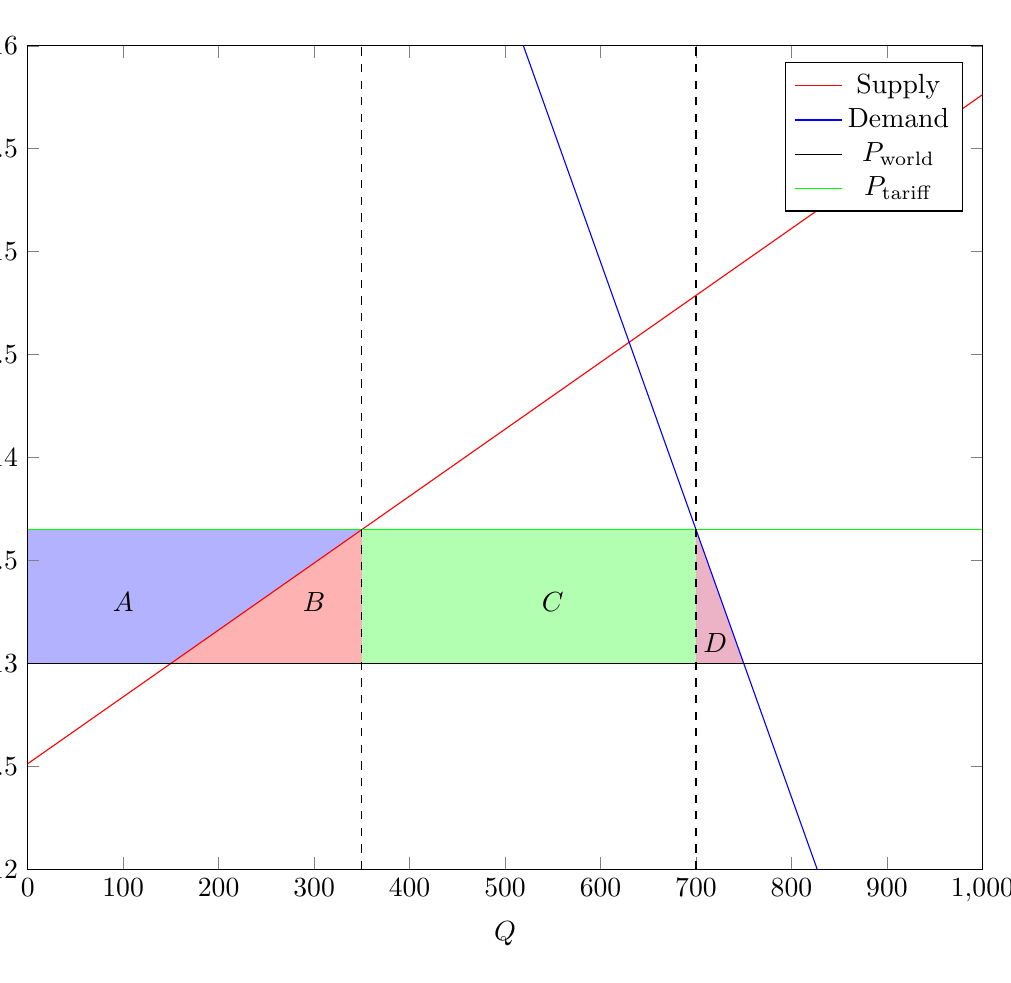
\begin{tikzpicture}
 	\begin{axis}[
	   xmin = 0, xmax = 1000,
	   ymin = 12, ymax = 16,
	   xlabel=$Q$,
	   ylabel=$P$,
	  ]
	  \addplot[name path global=supply, domain=0:1000, red] { 0.00325*x + 12.5125 };
	  \addplot[name path global=demand, domain=0:1000, blue] { -0.013*x + 22.75 };
	  \addplot[name path global=world, domain=0:1000, black] { 13 };
	  \addplot[name path global=tariff, domain=0:1000, green] { 13.65 };
	
	
	  \node at (axis cs:100, 13.3) {$A$};
	  \node at (axis cs:300, 13.3) {$B$};
	  \node at (axis cs:550, 13.3) {$C$};
	  \node at (axis cs:720, 13.1) {$D$};
	
	  \vasymptote[dashed]{350}{first}
	  \vasymptote[dashed]{700}{second}
	
	  \legend{Supply, Demand, $P_\mathrm{world}$, $P_\mathrm{tariff}$}
	
	  \path [name intersections={of=supply and world, by={a}},
	         name intersections={of=supply and tariff, by={b}},
	         name intersections={of=first and world, by={c}},
	         name intersections={of=second and world, by={d}},
	         name intersections={of=demand and tariff, by={e}},
	         name intersections={of=demand and world, by={f}}];
	
	 \begin{scope}[on background layer]
		\fill [blue,opacity=.3] (axis cs:0,13) -- (axis cs:0,13.65) -- (b) -- (a) -- cycle;
		\fill [red,opacity=.3] (a) -- (b) -- (c) -- cycle;
		\fill [green,opacity=.3] (b) -- (c) -- (d) -- (e) -- cycle;
		\fill [purple,opacity=.3] (e) -- (d) -- (f) -- cycle;
	 \end{scope}
 \end{axis}

\end{tikzpicture}

\end{document}